\begin{frame}{反力のチェックサム(設定)}
 
  PrePoMaxにおいて、反力チェックサムを確認するには、以下設定する \\
  % 図の挿入
  \begin{figure}[htbp]
    \begin{center}
      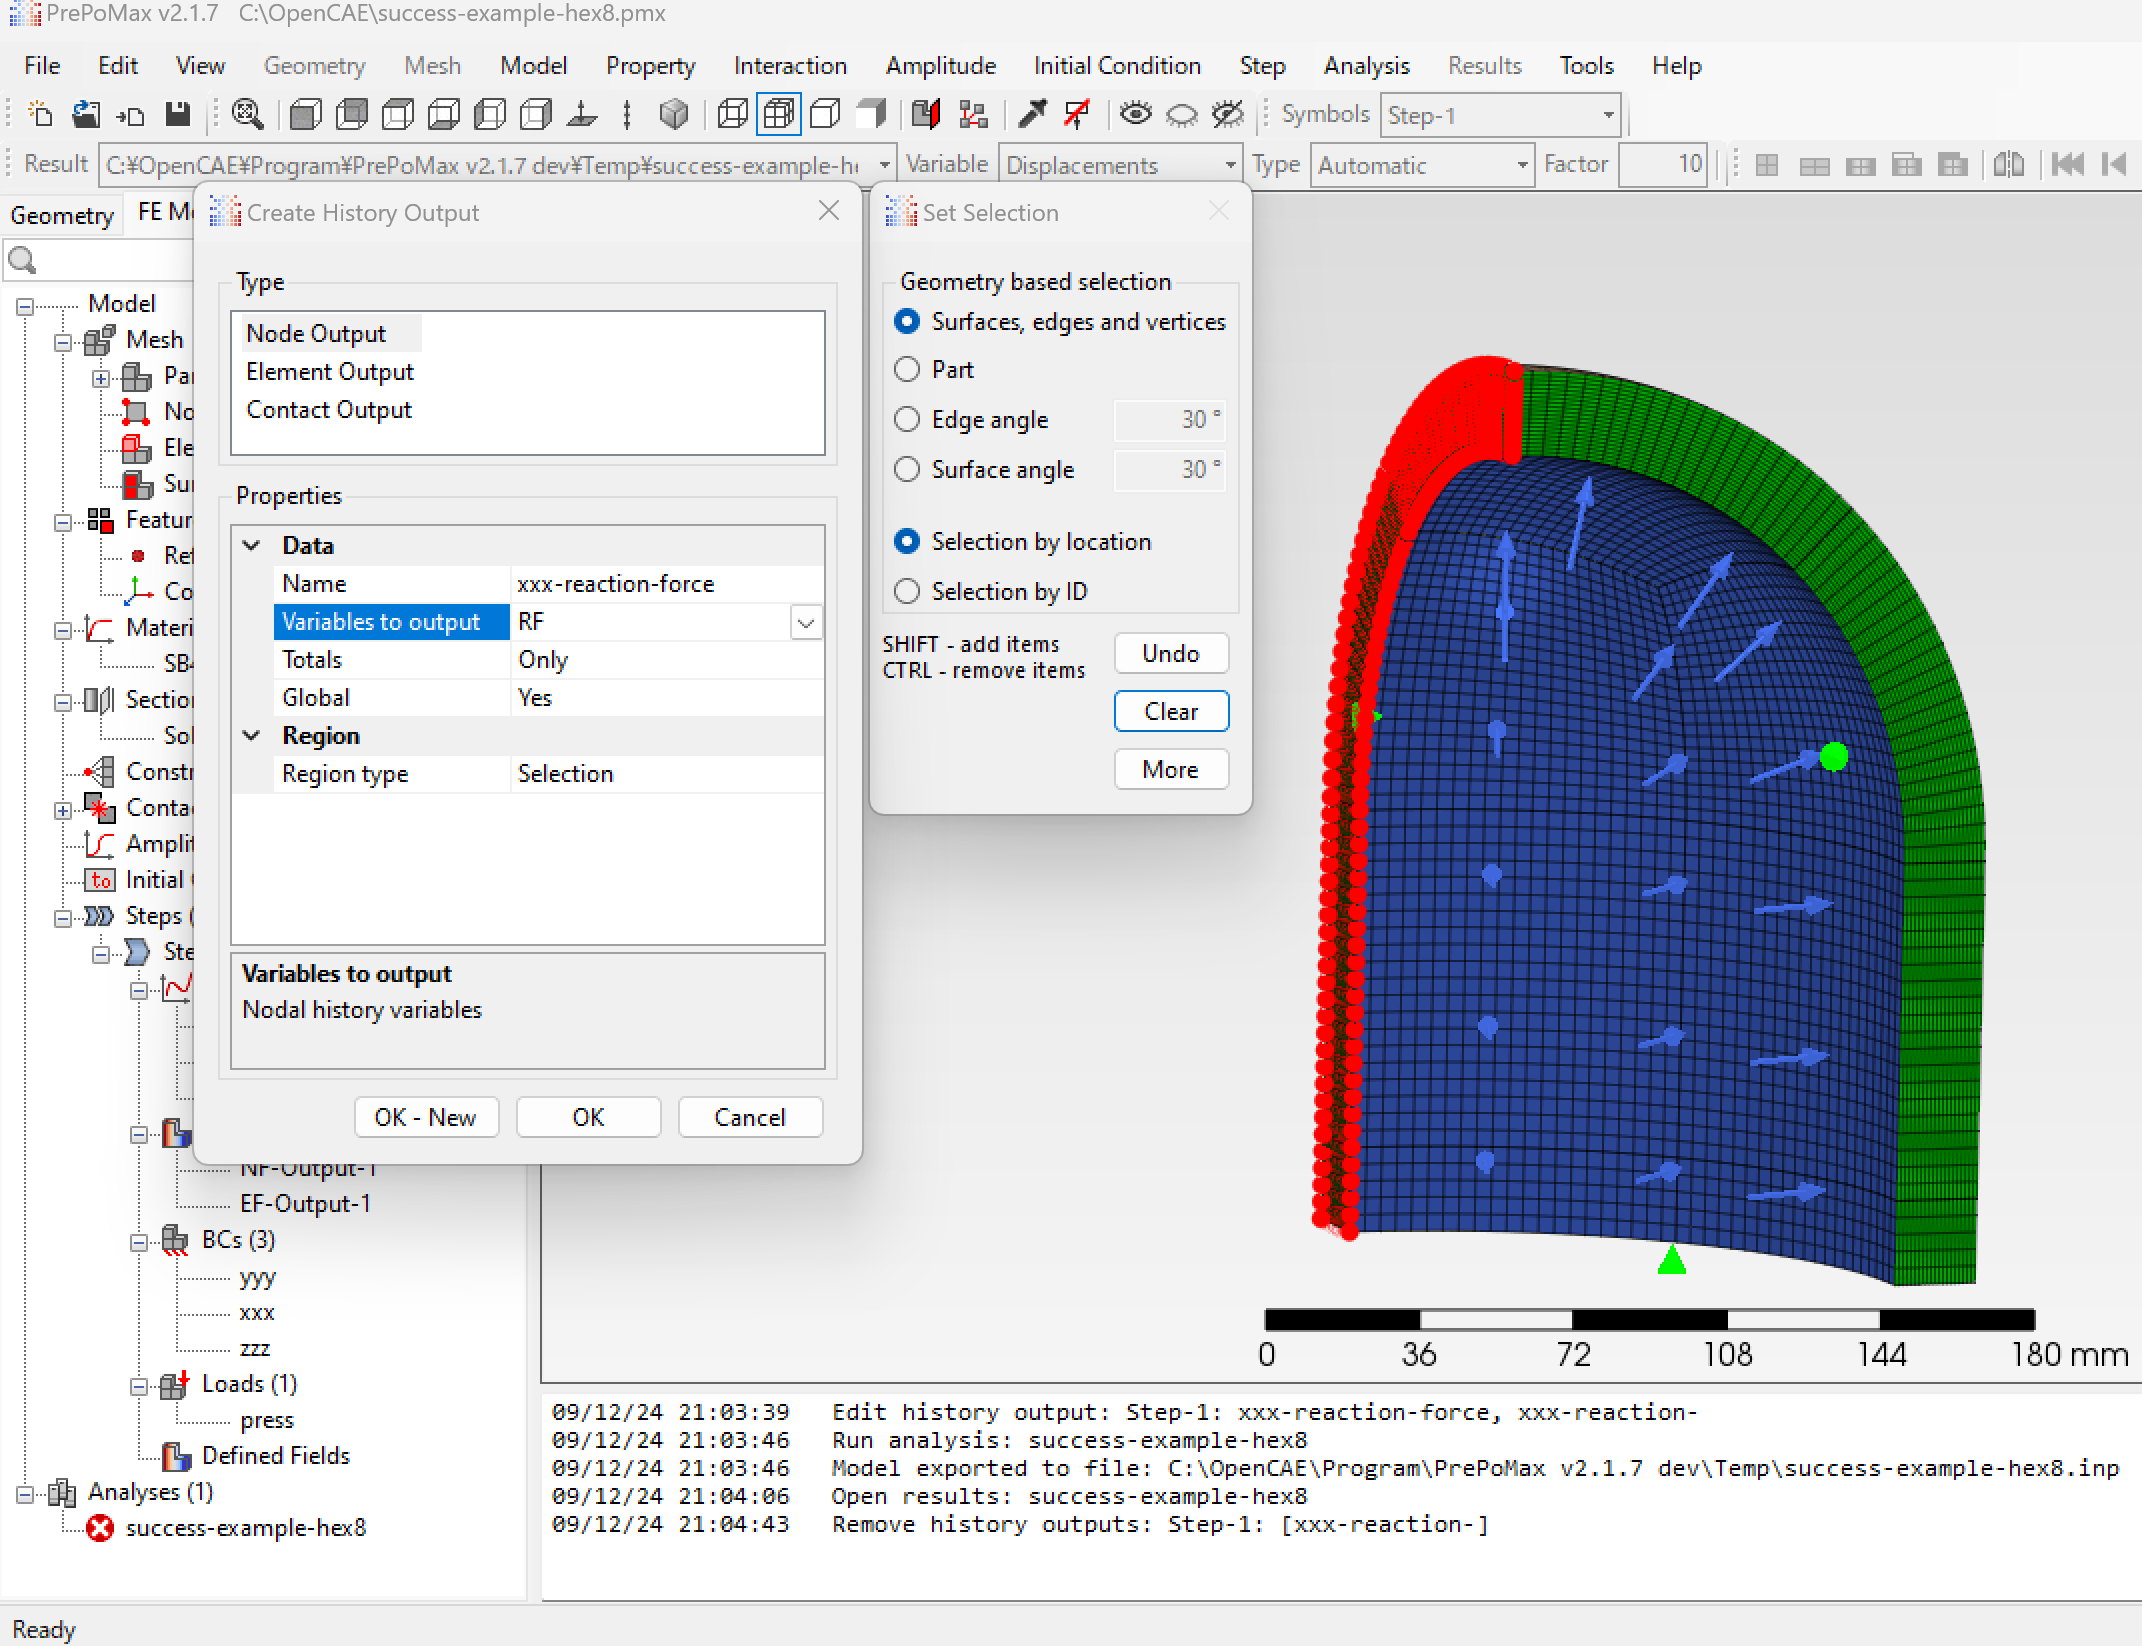
\includegraphics[keepaspectratio,scale=0.285]{images/screen01.png}
      \caption{反力チェックサムの設定}
    \end{center}
  \end{figure}
  \begin{textblock*}{160pt}(0pt,77pt)
    \begin{tikzpicture}
      \node[rectangle,fill=cud_yellow,text width=90pt,text centered,rounded corners,minimum height=20pt](s) at (1cm,1cm) { \scriptsize Node Output設定};
      \draw[->, draw=cud_red, line width=1pt] (80pt,28pt) -- (117pt,32pt);
    \end{tikzpicture}
  \end{textblock*}
  \begin{textblock*}{160pt}(0pt,110pt)
    \begin{tikzpicture}
      \node[rectangle,fill=cud_yellow,text width=90pt,text centered,rounded corners,minimum height=40pt](s) at (1cm,1cm) { \scriptsize 出力を\\「RF」に設定};
      \draw[->, draw=cud_red, line width=1pt] (80pt,28pt) -- (121pt,42pt);
    \end{tikzpicture}
  \end{textblock*}
  \begin{textblock*}{160pt}(0pt,120pt)
    \begin{tikzpicture}
      \node[rectangle,fill=cud_yellow,text width=90pt,text centered,rounded corners,minimum height=40pt](s) at (1cm,1cm) { \scriptsize Totalsを\\「Only」に設定};
      \draw[->, draw=cud_red, line width=1pt] (80pt,28pt) -- (121pt,85pt);
    \end{tikzpicture}
  \end{textblock*}
\end{frame}
